% TODO:
%   - Title spelling etc
%   - Kijk na of titels in header overflowen
% ----------  
% Questions:
%   - XXX



% Uncomment this if the use of parts is desired
\part{Reflection on the results of this master thesis}
\label{part:reflection}

% Will need a new title since it is no longer a system to use
\chapter{Evaluation of the proposed pipelines}
\label{ch:evaluation}

% ---------------------------------------------- 
% INTRODUCTION
% ---------------------------------------------- 
\section{Introduction to this chapter}
\label{sec:evaluation_introduction}
% NOTE: "Introduction" exists in each chapter and gives a short intro to the chapter + what can be expected in the chapter

The previous chapters discussed in great detail which \gls{mi} \gls{eeg} classification pipelines were considered for this master thesis, how they work and how they can be evaluated.
This chapter details the performed evaluations and the results obtained.
In particular, three main test settings were used: intrasession, intersession and intersubject evaluation.
Besides providing an overview of the obtained evaluation metrics, some reasoning into why certain experiments were performed and why certain results were expected is also given.
The used open-source \gls{mi} \gls{eeg} dataset is also briefly discussed.
Most experiments revolve around offline \gls{mi} \gls{eeg} classification performance, as this is the focus of this master thesis.
Some pilot experiments regarding recommended changes for going to an online setting discussed in Chapter \ref{ch:online_bci_system} were also performed and are also discussed in this section.

% ---------------------------------------------- 
% USED DATA
% ---------------------------------------------- 
\section{Three class MI EEG data source}
\label{sec:evaluation_data_source}

Following this master thesis' proposal of splitting \gls{bci} development in at least four distinct papers (Section \ref{subsec:bci_opportunities_obstacles_lack_of_testing}), this master thesis focusing on the classification pipeline should provide a summary of the data used.
The \gls{mi} \gls{eeg} data used for this master thesis is from an open-source dataset by \citet{eeg_data}.
\Citet{eeg_data} provide four different types of \gls{mi} interaction tasks, of which this master thesis works with the three class \gls{mi} \gls{eeg} dataset provided as the "CLA" dataset.

The hardware used for the data acquisition of this dataset uses the international 10-20 system discussed in \ref{subsec:biomedical_signals_working_with_eeg_standards}.
The used \gls{eeg} equipment makes use of wet electrodes and a sampling rate of 200\gls{hz}.
The participants were seated in a comfortable position throughout the experiment and remained motionless throughout the recordings, with a fixed gaze-fixation point to limit the presence of muscle artefacts which were discussed in Section \ref{subsec:biomedical_signals_working_with_eeg_artefacts}.
The provided data is band-pass filtered to include the frequencies between 0.53\gls{hz} and 70\gls{hz}.
A band-stop filter was also in place to remove \gls{ac} artefacts as discussed in Section \ref{subsec:biomedical_signals_working_with_eeg_artefacts}.
All of these frequency filters are hardware filters directly integrated into the hardware of the EEG-1200 hardware used for data acquisition.

The recordings of the CLA dataset provides balanced sampels of three \gls{mi} tasks reffered to as left-hand \gls{mi}, right-hand \gls{mi} and neutral \gls{mi}.
For the left-hand and right-hand \gls{mi} tasks, the participants were asked to imagine closing and opening the respective fist once.
For the neutral \gls{mi} task, the patient was asked to perform no \gls{mi}.
The communication of which task to perform was done via a simple graphical interface.
Upon showing the icon for which task to perform (event onset), the subject should perform the specific \gls{mi} task.
The icon is visible on the screen for one second past the event onset.
A random resting period of 1.5 to 2.5 seconds was present between the event offset and the event onset of a new task.
This process was repeated for 15 minutes, after which a longer resting period was present where it was ensured the \gls{eeg} equipment remained properly seated.
In total, three 15-minute trials were performed in one session.
This resulted in roughly 300 samples for each \gls{mi} task for each session.
Some subjects only had one recorded session whilst others had up to three.
All subjects were healthy, between 20 and 35 years old and living in Turkey.
No specific survey was performed to test the \gls{mi} capabilities beforehand nor does \citet{eeg_data} describe that any specific \gls{mi} training happened.

For the experiments of this master thesis, only subjects B, C and E of the CLA dataset were considered.
The motivation for this is them being the only ones with three different sessions available.
Given that there is no mention of \gls{mi} training by \citet{eeg_data}, it was reasoned that those who did three sessions would likely be better at \gls{mi}, especially in their last session.
Given the experience and feedback from two previous trials, it was also reasoned these subjects would create fewer muscle artefacts that could be unwillingly used for learning, such as those discussed in Section \ref{subsec:biomedical_signals_working_with_eeg_artefacts}.
As such, the test sessions for these subjects were always the last recorded session for the experiments of this master thesis.

The data from the CLA dataset is provided as MatLab files originally.
To make them usable in Python, the experimental notebooks provided on the GitHub repository of this project provide conversion methods to convert these MatLab files to MNE Raw objects \citep{github_project, mne}.
To facilitate the use of this dataset in Python for other researchers, the GitHub repository also provides the CLA dataset as \gls{fif} files.
These \gls{fif} files can be easily opened with MNE Python and include all provided details by \citet{eeg_data} stored in the associated info object.
The utility file $\texttt{CLA\_dataset.py}$ provides many functions for working with this CLA dataset in Python.

% ---------------------------------------------- 
% GENERAL REMARKS
% ---------------------------------------------- 
\section{General remarks on experiment setups}
\label{sec:evaluation_general_remarks}

To provide the best possible reproducibility all resources needed to recreate the empirical evaluation results are available on the documented GitHub repository of this master thesis \citep{github_project}.
This includes saved weights of the exact models used for the results discussed in this chapter and many utility files to facilitate loading and working with these models.

All training and testing was done on a 64-bit Windows 10 Pro machine with an Intel Core i5-4690K overclocked at 4.2GHz.
An MSI NVIDIA GeForce GTX970 \gls{gpu} was used in the training of the \gls{dl} models with CUDA support through the CuDNN 8.2.2 driver.
The system in question had 16GB of ram, of which an approximate 10GB was usable for the training procedure.
These specifications allowed for sufficient training of the two-step \gls{ml} and state-of-the-art \gls{cnn} models in a reasonable time.
The longest cross-validated grid search hyperparameter tuning experiment for the two-step \gls{ml} approaches took around 30 hours to finish.
The longest experiment for the literature proposed \gls{cnn} models was finished in less than 6 hours.
The \gls{lstm} models were computationally heavy, and the convolutional \gls{lstm} extension to EEGNet does not have CUDA support.
This resulted in longer training times, with manageable times of under 6 hours for the regular \gls{lstm} extended EEGNet model.
However, for the convolutional \gls{lstm} extend EEGNet model, certain configurations were not possible due to limited video RAM and fewer epochs were performed for training.
The latter didn't seem to influence the results as the evolution of both training and validation accuracy and loss converged in all experiments.
These metrics were closely monitored during all training of the \gls{dl} methods to ensure no overfitting tendencies are present.
En example of validation loss and accuracy evolution is given in Figure \ref{fig:results_tensorboard}.

The used representation of the \gls{eeg} signal provided through MNE makes use of extremely small values.
This causes issues for the \gls{dl} approaches and as such the data was first multiplied by 1000000 before using it in the \gls{dl} classification pipelines.
Each experiment made use of a fixed length window around a known event as described in Section \ref{subsec:processing_signals_general_pipeline_windowing}.
Two window lengths were considered, a 0.5-seconds window used for all experiments and a longer 1.5-second window additionally tested for most experiments.
The 0.5 seconds window started 0.1 seconds after the event onset and ended 0.6 seconds after the event onset.
The 1.5 seconds window started 0.25 seconds before the event onset and ended 1.25 seconds after the event onset.
This chapter discusses the results of the 0.5-seconds unless stated otherwise.

The traditional two-step \gls{ml} approaches made use of cross validated gridsearch hyperparameter tuning to find the best possible combination of parameter settings, as discussed in Section \ref{subsec:offline_bci_system_two_step_ml_basic_csp}.
Due to the computational power that would be needed to perform such a cross-validated grid search for hyperparameter tuning of the \gls{dl} methods, parameters were chosen based on the literature proposed configurations and finetuned based on pilot studies performed in the experimental notebooks.
This also means that whilst the traditional two-step \gls{ml} approaches mostly have 4-fold validation accuracy reported together with their standard deviation, the \gls{dl} models only have a singular validation accuracy available obtained from a typical 20\% split during Keras training.

The \gls{dl} models were trained for sufficient epochs, 250 to 2500 dependent on the data and pipeline, where both training scores and validation scores on basis of accuracy and loss were monitored to ensure stable training.
For each training procedure of the \gls{dl} models, two variants of the model were saved.
One where the validation loss was lowest and one where the validation accuracy was the highest.
These variants are used for obtaining the final results on the test sets, which were equal for all models and 20\% of the total available data.
The best variant of these two is the one reported in this chapter.
Due to the use of balanced data, the accuracy of a random model would be $\frac{1}{3}$ in all experiments.

\begin{figure}[ht]
    \centering
    \begin{subfigure}{0.9\textwidth}
        \centering
        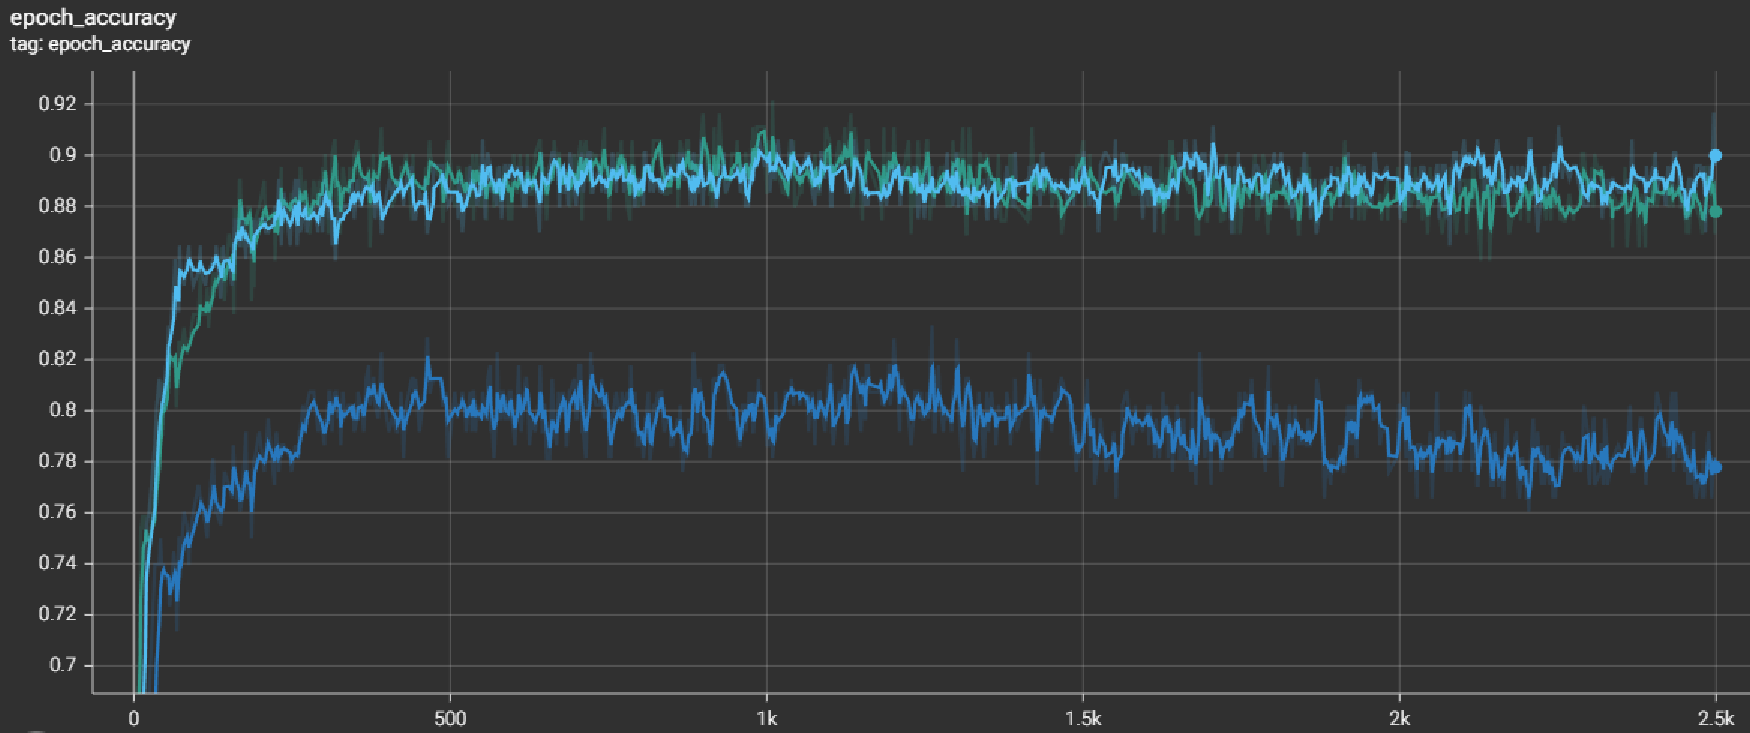
\includegraphics[width=\textwidth]{../images/results/accuracy.pdf}
        \captionsetup{width=\linewidth}
        \captionsetup{justification=centering}
        \caption{Evolution of validation accuracy over time.}
        \label{fig:results_tensorboard_acc}
    \end{subfigure}
    \hfill
    \vfill
    \begin{subfigure}{0.9\textwidth}
        \centering
        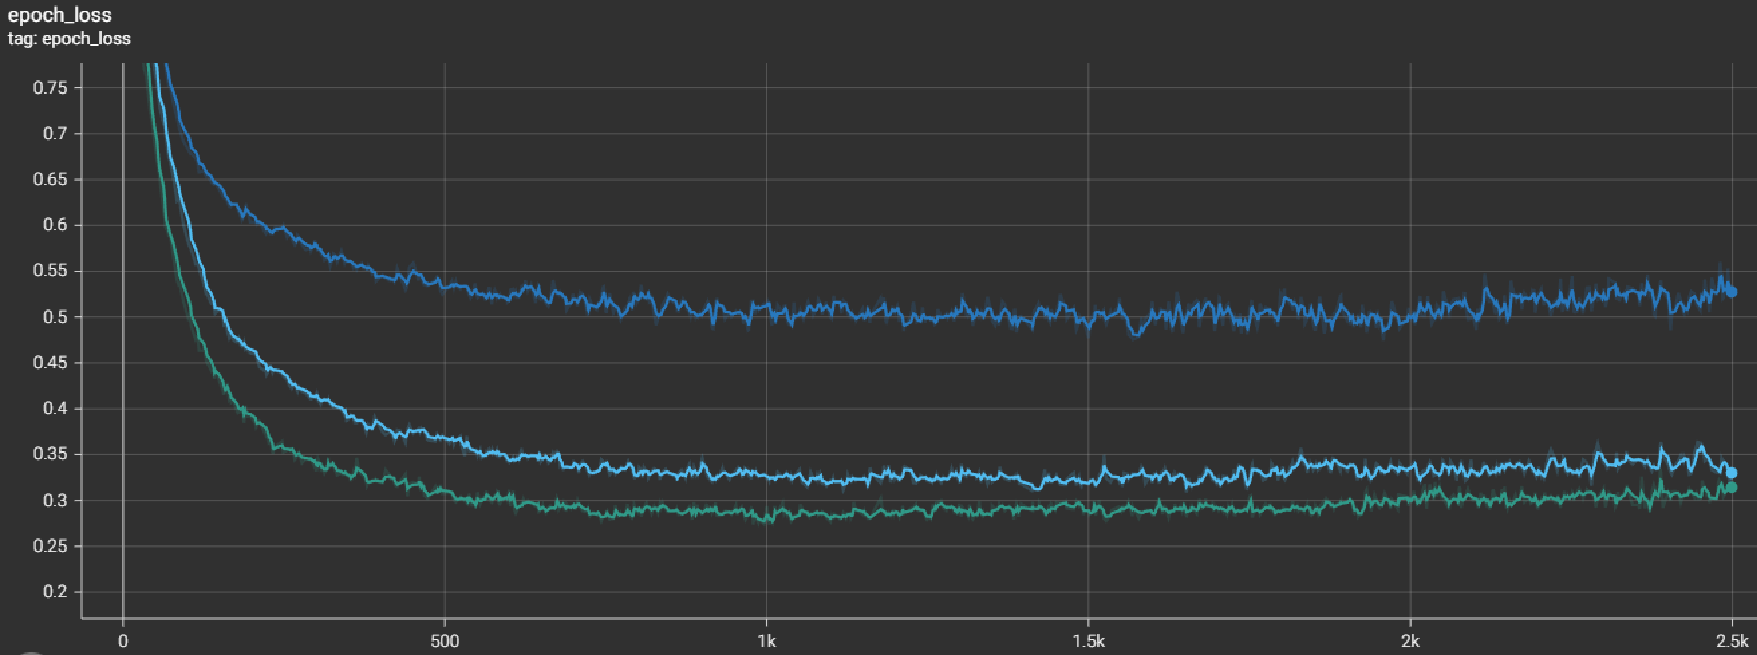
\includegraphics[width=\textwidth]{../images/results/loss.pdf}
        \captionsetup{width=\linewidth}
        \captionsetup{justification=centering}
        \caption{Evolution of validation loss over time.}
        \label{fig:results_tensorboard_loss}
    \end{subfigure}
    \captionsetup{width=\linewidth}
    \captionsetup{justification=centering}
    \caption{Evolution of both validation accuracy and validation loss over time. Graphs shown are from the intrasession experiment of EEGNet for subjects B (dark blue), C (light blue) and E (green). The time axis denotes the epoch in which the result is obtained.}
    \label{fig:results_tensorboard}
\end{figure}

These general remarks should suffice for a precise understanding of the results discussed in the remainder of this chapter.
As discussed, all learned models and the code for all performed experiments is available on the GitHub repository of this master thesis to ensure complete reproducibility \citep{github_project}.

% ---------------------------------------------- 
% CONSIDERED EVALUATION METRICS
% ---------------------------------------------- 
\section{Considered evaluation metrics}
\label{sec:evaluation_eval_metrics}

Considering the goal of these \gls{mi} \gls{eeg} classification pipelines is to ultimately be used in a \gls{bci} application, reporting on the validation and/or testing accuracy alone doesn't tell that much.
From the alternatives provided in Section \ref{subsec:processing_signals_evaluating_and_using_evaluation}, three additional metrics derived from the test set's \gls{cm} are discussed for the main experiments of this master thesis.
The first two provide the \gls{ppv} for both left-hand and right-hand \gls{mi} class labels.
These metrics are interesting, as they provide insight into how many times an action linked to this label would be performed with the user's intent.
By doing so, it also directly provides how many times an action was taken without the user's intent, as this is just 100\% - the metric.
The higher this metric, the better the model is in this regard.
As a more general idea of how many times the system would make a \textit{risky error}, another metric is also proposed.
This metric represents how many times either the left-hand or right-hand \gls{mi} class label is wrongly predicted out of all predictions.
A lower value thus denotes a better model in this regard.
The best performing model in each of these metrics has its score for the metric in bold.
All of the \glspl{cm} used to obtain these results can be found on the GitHub repository of this master thesis \citep{github_project}.


% ---------------------------------------------- 
% INTRA SESSION
% ---------------------------------------------- 
\section{Intrasession evaluation}
\label{sec:evaluation_intrasession}


\begin{figure}[!p]
    \centering
    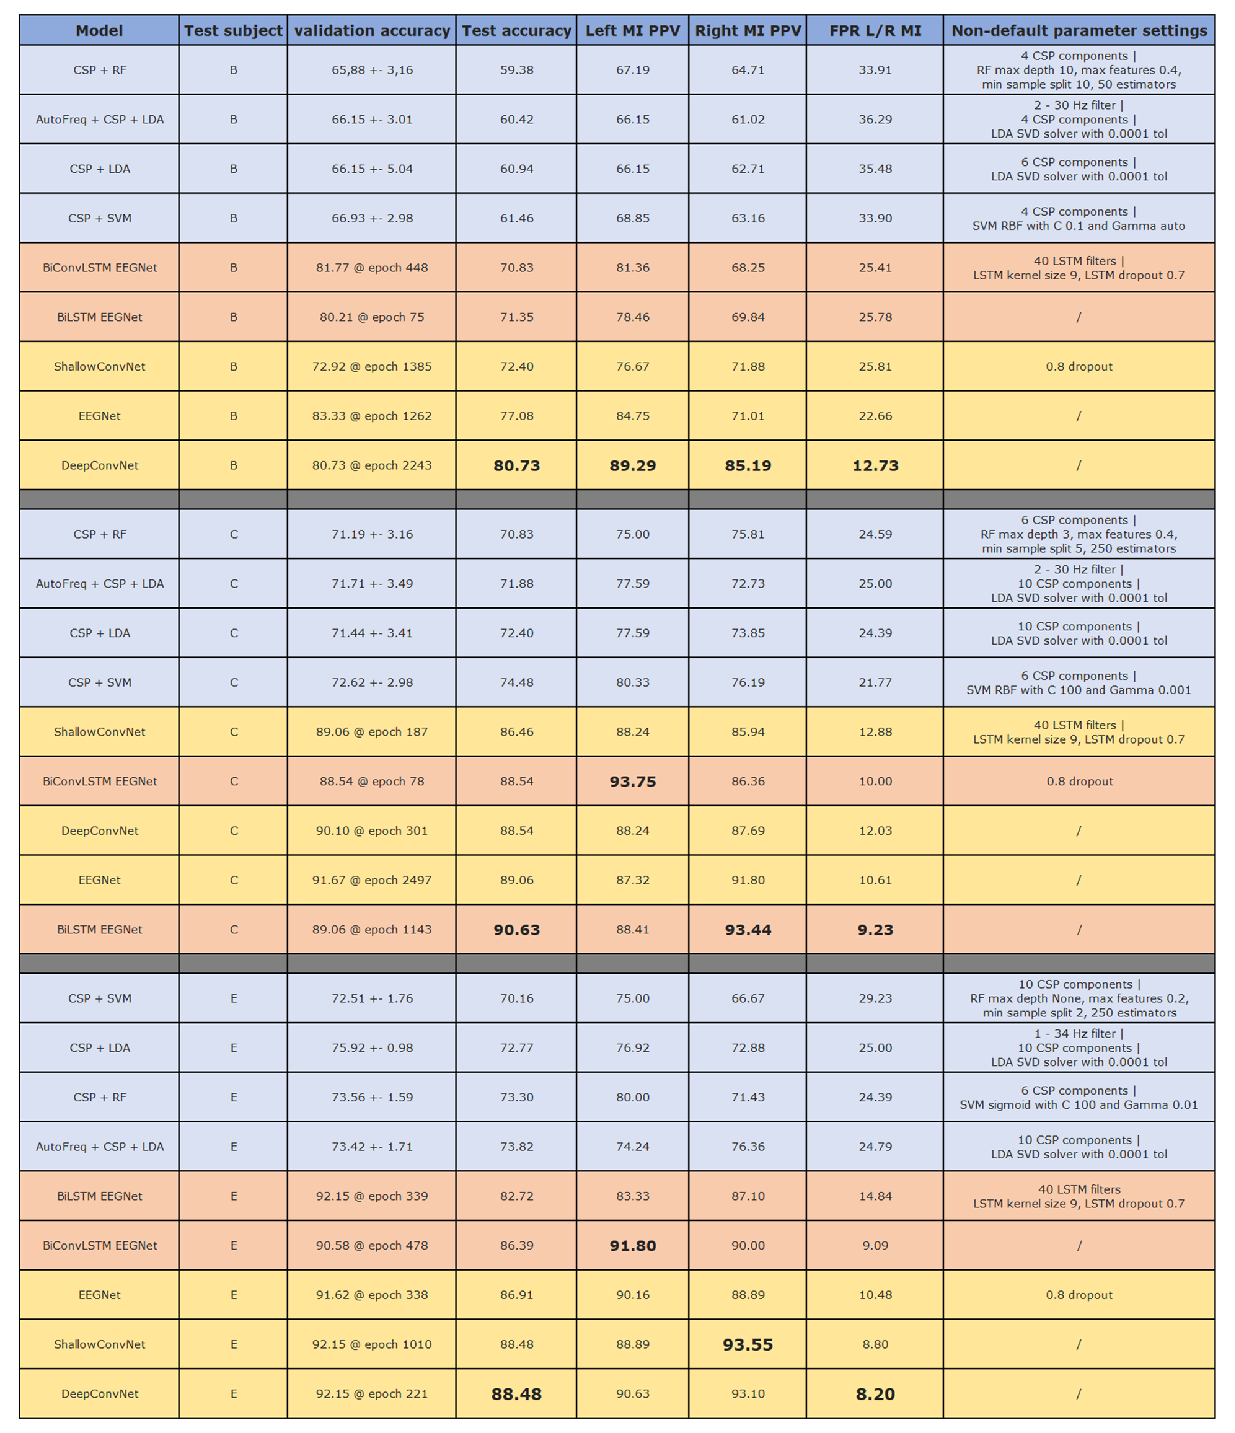
\includegraphics[width=\linewidth]{../images/results/intrasession.pdf}
    \captionsetup{width=\linewidth}
    \captionsetup{justification=centering}
    \caption{Intrasession results for all classification approaches. Results are sorted based on the test subject and the obtained classification result on the test set. Colour codes denote either two-step \gls{csp} approaches, literature proposed \gls{cnn} approaches or master thesis proposed \gls{cnn}-\gls{lstm} approaches.} 
    \label{fig:results_intrasession}
\end{figure}


The first experimental setup consisted of an intrasession evaluation.
For such an experiment, each classification pipeline is trained and tested on \gls{mi} \gls{eeg} data from the same subject and the same session.
This experimental setup is the easiest to learn as it is least influenced by the generalisability issues of \gls{mi} \gls{eeg} data discussed in Section \ref{subsec:biomedical_signals_working_with_eeg_generalisation}.
Whilst in other fields this approach would be considered data leakage, a phenomenon discussed in Section \ref{subsec:processing_signals_evaluating_and_using_evaluation}, it is a relatively common setup for this kind of research.
The main defence for this is that most real-world applications of \gls{mi} require up to 20 minutes of calibration anyway \citep{eeg_model_eegnet}.
The models are trained on 60\% of the data, validated on 20\% of the data for finding the best parameter configurations and tested on the test set consisting of 20\% of the data.

Figure \ref{fig:results_intrasession} summarizes all obtained results in terms of validation and test accuracy along with the three other \gls{cm} derived metrics discussed in Section \ref{sec:evaluation_eval_metrics}.
Given the limited amount of training data, around 200 samples per class, a reasonable assumption would be to think that a deep \gls{dl} model such as DeepConvNet would overfit and perform poorly on the test set and that a shallow \gls{dl} model such as ShallowConvNet would perform better.
However, given the test set is from the same subject in the same session, the test data matches the training data especially well and DeepConvNet is the most consistent approach in terms of accuracy.
It has a mean test accuracy of $85.92$ with a standard deviation of ± $3.67$ compared to ShallowConvNet's $82.45$ ± $7.15$.
It is noteworthy that subject B seems to be more difficult to learn compared to the other two subjects.
This finding is consistent between all experiments and could potentially be related to the subject's \gls{mi} capabilities.
However, since no survey to test these capabilities was performed by \citet{eeg_data}, it can't be validated.

All the \gls{dl} models outperform the two-step \gls{csp} approaches.
However, given the simplicity of \gls{csp}, the obtained results are still pleasant and extensions such as \gls{fbcsp} are expected to perform even better.
With a risky error below 10\% for all patients when using DeepConvNet, and having a \gls{ppv} for both left and right-hand classes, the model could have great potential for use in a comparable \gls{bci} setting.
Multiple tricks, such as requiring multiple successive classifications of the same class before acting, can help in reducing the risky error even more but fall outside the scope of this master thesis.




% ---------------------------------------------- 
% INTER SESSION
% ---------------------------------------------- 
\section{Intersession evaluation}
\label{sec:evaluation_intersession}


\begin{figure}[!p]
    \centering
    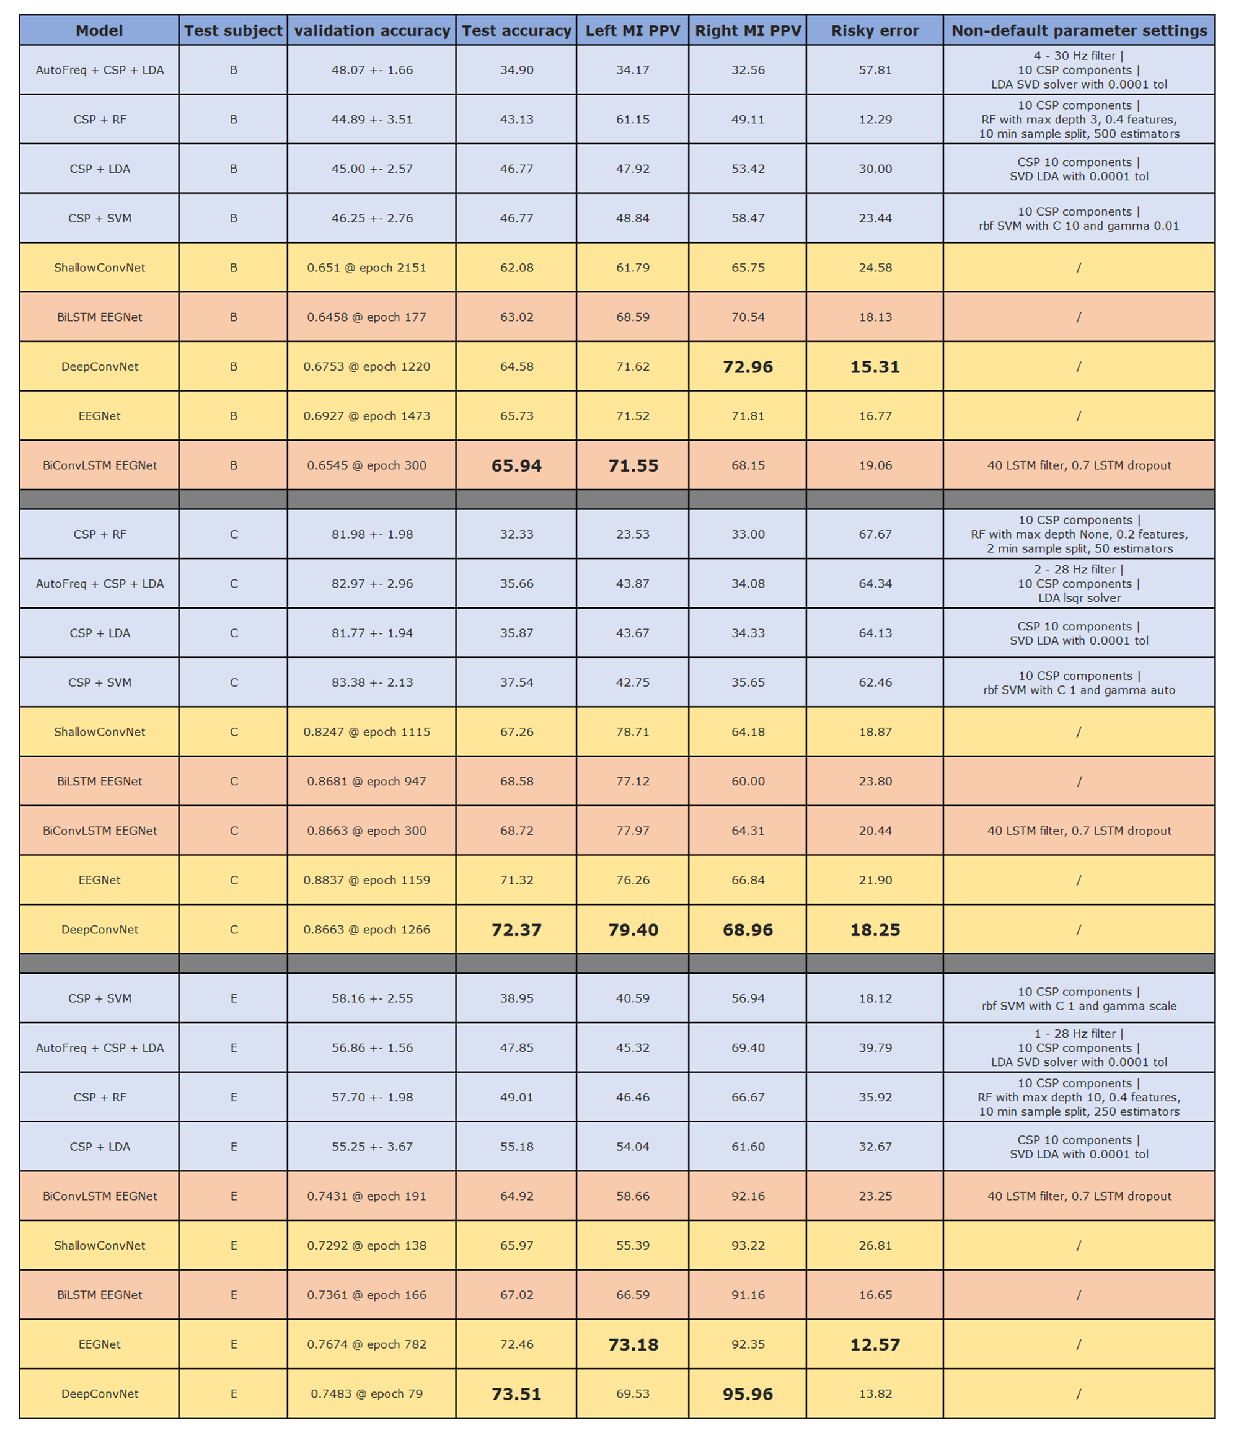
\includegraphics[width=\linewidth]{../images/results/intersession.pdf}
    \captionsetup{width=\linewidth}
    \captionsetup{justification=centering}
    \caption{Intersession results for all classification approaches. Results are sorted based on the test subject and the obtained classification result on the test set. Colour codes denote either two-step \gls{csp} approaches, literature proposed \gls{cnn} approaches or master thesis proposed \gls{cnn}-\gls{lstm} approaches.} 
    \label{fig:results_intersession}
\end{figure}

The second experimental setup is more representative of a real-world application.
By training on the first two sessions of a subject and testing on the third, an intersession evaluation is performed.
It is noted that both sessions were used as training data, with a subsample of both being used as validation data.
A more representative validation strategy would be to use one session as training data and one as validation data.
However, this would limit the training set to one session, for which it is reasoned that the generalisability of the model will suffer due to it not having access to different sessions and thus a greater variety of data.
Following this reasoning, which was further supported by a pilot study, it was chosen to use 60\% of both sessions as training data,  20\% as validation data and 20\% as test data.

Figure \ref{fig:results_intersession} summarizes all obtained results similar to the summary from the intrasubject experiment.
Both DeepConvNet and EEGNet perform equally well, with a mean test accuracy of $70.15$ ± $3.97$ and $69.84$ ± $2.94$ respectively.
The difference between EEGNet and the extension proposed is slim to none when looking at the metrics provided. 
Whilst both EEGNet and ShallowConvNet claimed to be inspired by the same \gls{fbcsp} approach that is known to perform well for these tasks, they differ significantly in some of the reported evaluation metrics.
This is most notable for subject E, where EEGNet has a risky error of less than half that of ShallowConvNet.
Likewise, the \gls{ppv} for left-hand \gls{mi} is significantly higher in favour of EEGNet.
This suggests that EEGNet makes most of its mistakes on the false passive \gls{mi} predictions, whereas ShallowConvNet does so on false left-hand \gls{mi} predictions.
This suggests that EEGNet and ShallowConvNet are learning different features.

The best-achieved test accuracy of $65.94$ for subject B, obtained by the bidirectional convolutional \gls{lstm} extension to EEGNet, is likely too low for most \gls{bci} applications, even with metrics in place to limit risky errors.
The test accuracies hovering around 73\% for the other two subjects, obtained by both DeepConvNet and EEGNet, are more promising in this regard and given some error-reducing metrics are in place, it would allow for use in \gls{bci} applications with no risks.

The traditional two-step \gls{ml} approaches using \gls{csp}-based feature extraction struggle at learning a generalizable model.
When looking at the difference between validation accuracy and test accuracy, especially notable for subject C, it is clear the models are overfitting.
Whilst this is a trend for all models on subject C, suggesting its last recording is less in line with its first two, it is extra apparent for the \gls{csp} approaches.
Their test accuracies obtained by the \gls{csp} methods for subject C are similar to that of random prediction (33\%).



% ---------------------------------------------- 
% INTER SUBJECT
% ---------------------------------------------- 
\section{Intersubject evaluation}
\label{sec:evaluation_intersubject}


\begin{figure}[!p]
    \centering
    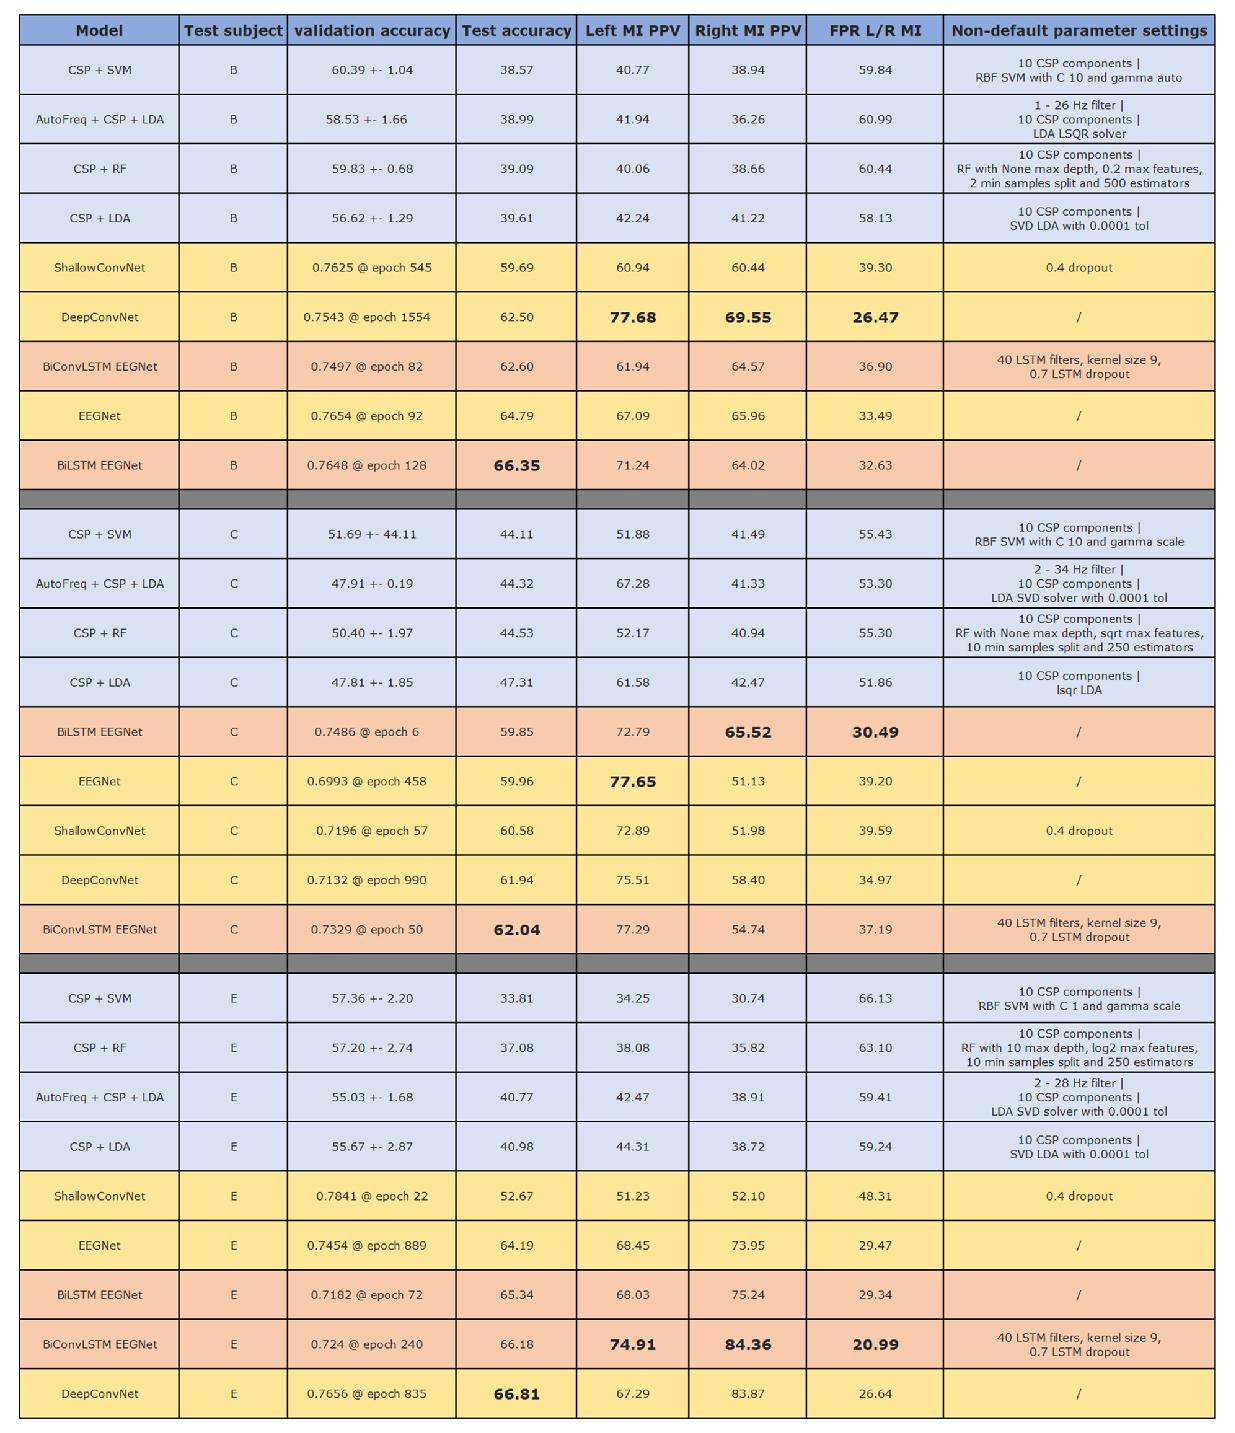
\includegraphics[width=\linewidth]{../images/results/intersubject.pdf}
    \captionsetup{width=\linewidth}
    \captionsetup{justification=centering}
    \caption{Intersubject results for all classification approaches. Results are sorted based on the test subject and the obtained classification result on the test set. Colour codes denote either two-step \gls{csp} approaches, literature proposed \gls{cnn} approaches or master thesis proposed \gls{cnn}-\gls{lstm} approaches.} 
    \label{fig:results_intersubject}
\end{figure}

The final and most difficult-to-learn experimental setup is an intersubject one, where the classification pipelines are tested on the last session of one subject and trained on all sessions of the other subjects.
Having a model that works even reasonably well in this experimental setup is considered a pleasing results as the common generalisability issues discussed in Section \ref{subsec:biomedical_signals_working_with_eeg_generalisation} and the more difficult nature of \gls{mi} classificiation discussed in Section \ref{subsec:biomedical_signals_working_with_eeg_inducing_methods} make this a complex task.

Like the reasoning provided for not keeping one of the two training sessions as a validation session, it is chosen to use both subjects in training and have a random sample split from this data as a validation split.
This is done since it was thought that opting to have a better validation strategy was expected to result in poorer performance due to the reduction in data.
Figure \ref{fig:results_intersubject} summarizes all obtained results similar to the summaries before.
With a mean test accuracy of $63.61$ ± $1.83$, the bidirectional convolutional \gls{lstm} extension to EEGNet performs best.
Whilst this is promising for the architecture proposed but this master thesis, it is without any statistical significance as the other \gls{lstm} extension, EEGNet and DeepConvNet hover around the same mean test accuracy with slightly larger standard deviations.

More interestingly, for neither of the three subjects is the classification pipeline with the best test set accuracy the one with the best score for any of the other \gls{cm} based metrics.
This further illustrates how accuracy alone doesn't provide much information.
This is especially noteworthy for the DeepConvNet model of subject B, where the misclassification rate for risky actions is almost twice as low compared to the \gls{cnn}-\gls{lstm} model which had the best test accuracy.
Whilst none of the pipelines are trained to favour false passive \gls{mi} misclassification, it is interesting to see that some models do this significantly more than others.

Another interesting finding is the EEGNet extended test accuracy obtained for subject B.
Not only is it the best for that subject, but it also outperforms the intersession results for that subject.
This illustrates that intersession variability for one subject can be incredibly high as it is more beneficial to learn from two distinct others to have more variable features extracted.
In summary, the intersubject accuracy obtained and the \gls{ppv} and risky errors provided are pleasing for most \gls{dl} models, but they are most likely too poor for use in an online \gls{bci} system.



% ---------------------------------------------- 
% LONGER WINDOW LENGTHS
% ---------------------------------------------- 
\section{Longer window lengths}
\label{sec:evaluation_longer_window_lengths}

\begin{figure}[ht]
    \centering
    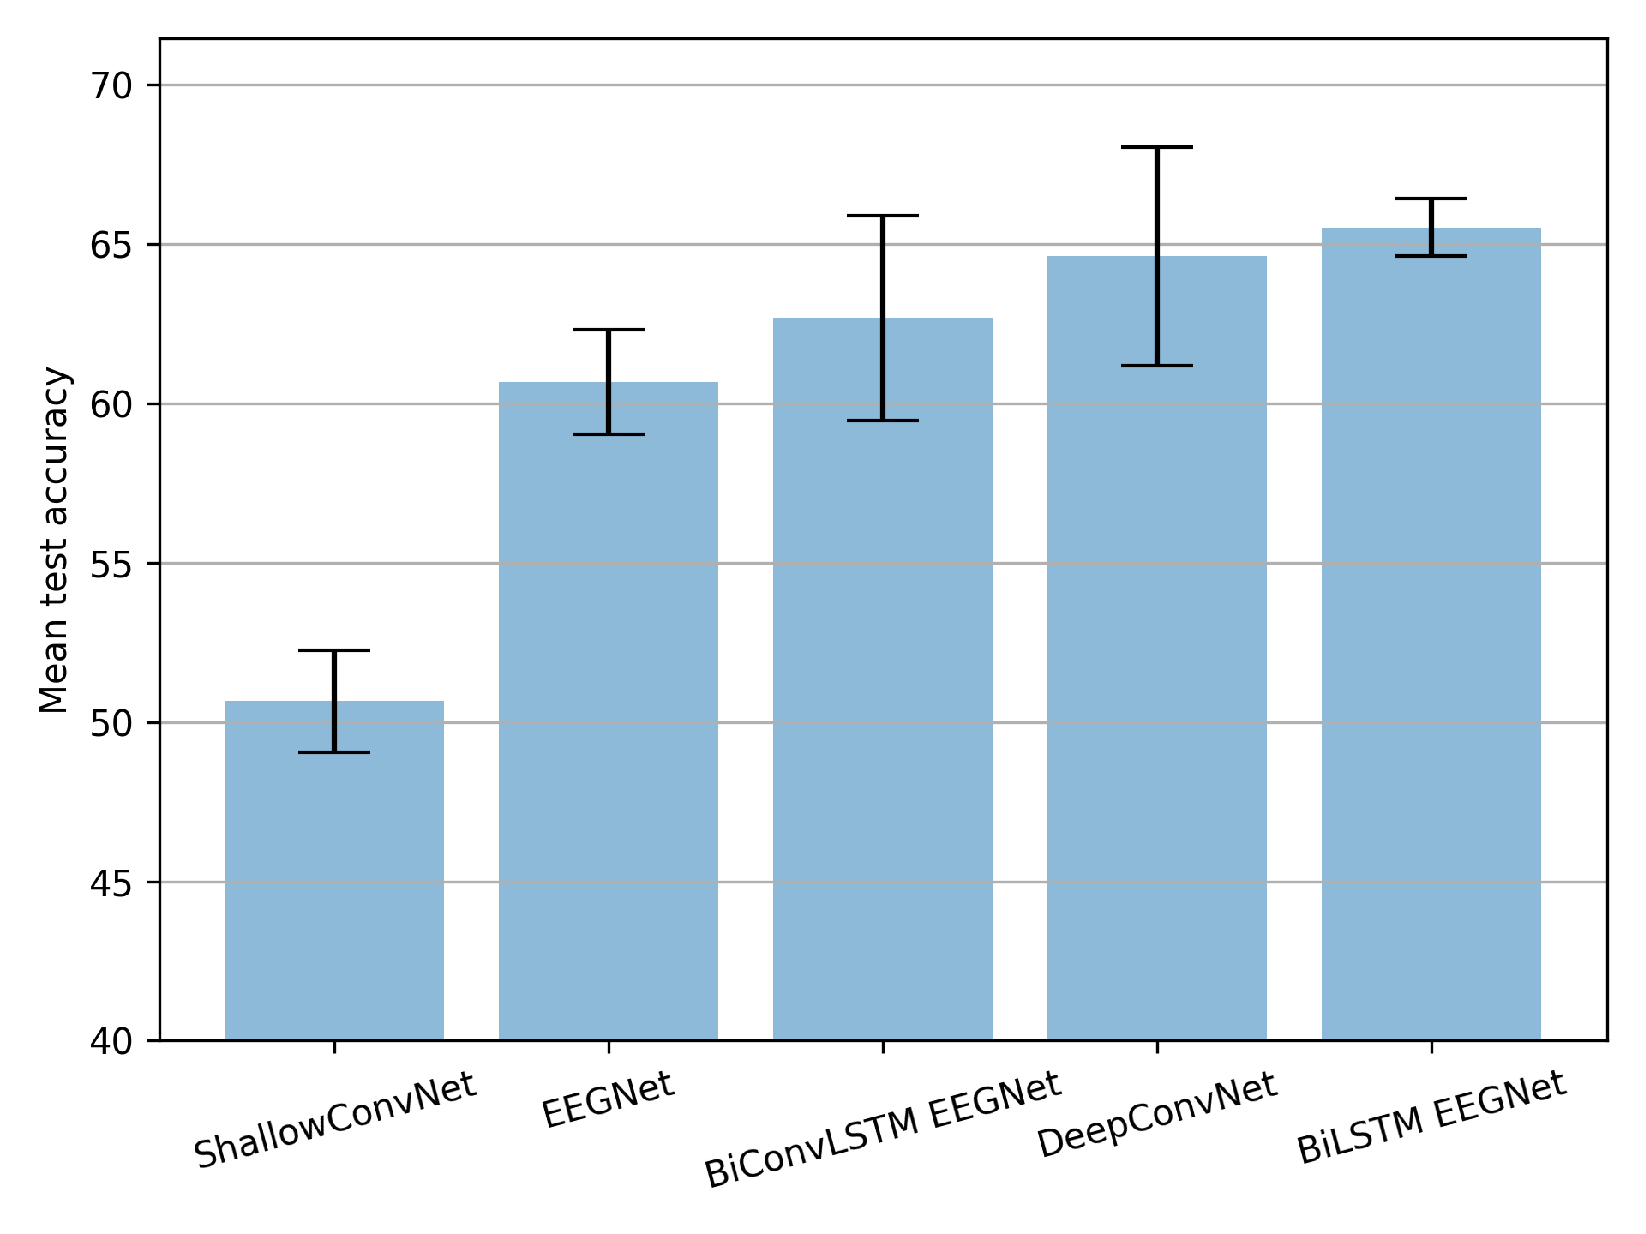
\includegraphics[width=0.5\linewidth]{../images/results/new_subject_longer_window.pdf}
    \captionsetup{width=\linewidth}
    \captionsetup{justification=centering}
    \caption{Mean test accuracies and their standard deviation from the longer window experiments in an intersubject evaluation setting.} 
    \label{fig:results_intersubject_long_bar}
\end{figure}

It was discussed in Section \ref{subsec:processing_signals_ml_and_dl_dl_classifiers} that networks using \gls{lstm} functionality are an interesting choice for time series such as \gls{eeg} and it was deemed possible an improvement could be seen.
However, none of the discussed main experiments provided statistically significant improvements for the extended EEGNet models over the base one.
When reflecting on the experimental setups, the use of a relatively short fixed window around the known event is likely the reason that added memory and sequence understanding doesn't have a significant benefit for the experiments.
With the windows starting 0.1 seconds after the event onset and being only 0.5 seconds long, it is unlikely for there to be unneeded segments of time that can be recognized by the \gls{lstm}.
Due to the fixed window location around the event and the relatively constant reaction speed expected from the participants, there are also no major timeshifts expected in the signal.
As such, the local patterns learned by the \gls{cnn} models whose relatively wide kernel goes over the temporal axis, are likely to capture all meaningful information.
Adding to this, the use of two convolutions over the time axis by EEGNet, the last convolutional layer using a downsampled and temporal feature extracted output of the first and second convolutional layer has access to a broader time range.
It could be argued that this also provides some forms of memory as it is looking for local patterns in data that is already feature extracted on a smaller time window for local patterns.

However, considering that the difference between the \gls{cnn} models and the \gls{lstm} extended EEGNet models became more favourable for the latter when complexity increased for the intersubject setting suggests that \gls{lstm} might be learning meaningful additional information.
As a first step to test this theory, a three times longer windowing technique was considered, starting 0.25 seconds before the onset and ending 1.25 seconds after the onset.
The summarized results of these longer window experiments are added to the extra figures list at the end of this master thesis.
An overall increase in performance for most models and metrics is seen throughout all experiments.
This suggests the half-second window doesn't capture all useful information.

Most interestingly are the intersubject experiments using these longer windows, the accuracy results of which are summarized in Figure \ref{fig:results_intersubject_long_bar}.
With a mean test accuracy of $65.52$ ± $0.89$, the \gls{lstm} extended EEGNet model performed better than the regular EEGNet model which had a mean test accuracy of $60.68$ ± $1.64$.
although this is only a first step in showing that the additional functionality of \gls{lstm} can be helpful, it is a promising one.
Further research into this classification approach, especially using sliding windows where temporal insight is even more important, could point to an even more significant finding than this initial one.





% ---------------------------------------------- 
% PILOT STUDIES
% ---------------------------------------------- 
\section{Additional pilot studies}
\label{sec:evaluation_pilot_studies}

Taking into consideration the steps of moving from an offline \gls{mi} \gls{mi} classification approach to an online \gls{bci} discussed in Chapter \ref{ch:online_bci_system}, some additional pilot studies were done.
Since these are pilot studies, they only aim to provide a deeper insight into the discussed proposals and an indication of what can be expected from future research.

% - - - - - - - - - -
% more data
% - - - - - - - - - -
\subsection{Improving intersubject performance by providing more data}
\label{subsec:evaluation_pilot_studies_more data}

\begin{figure}[ht]
    \centering
    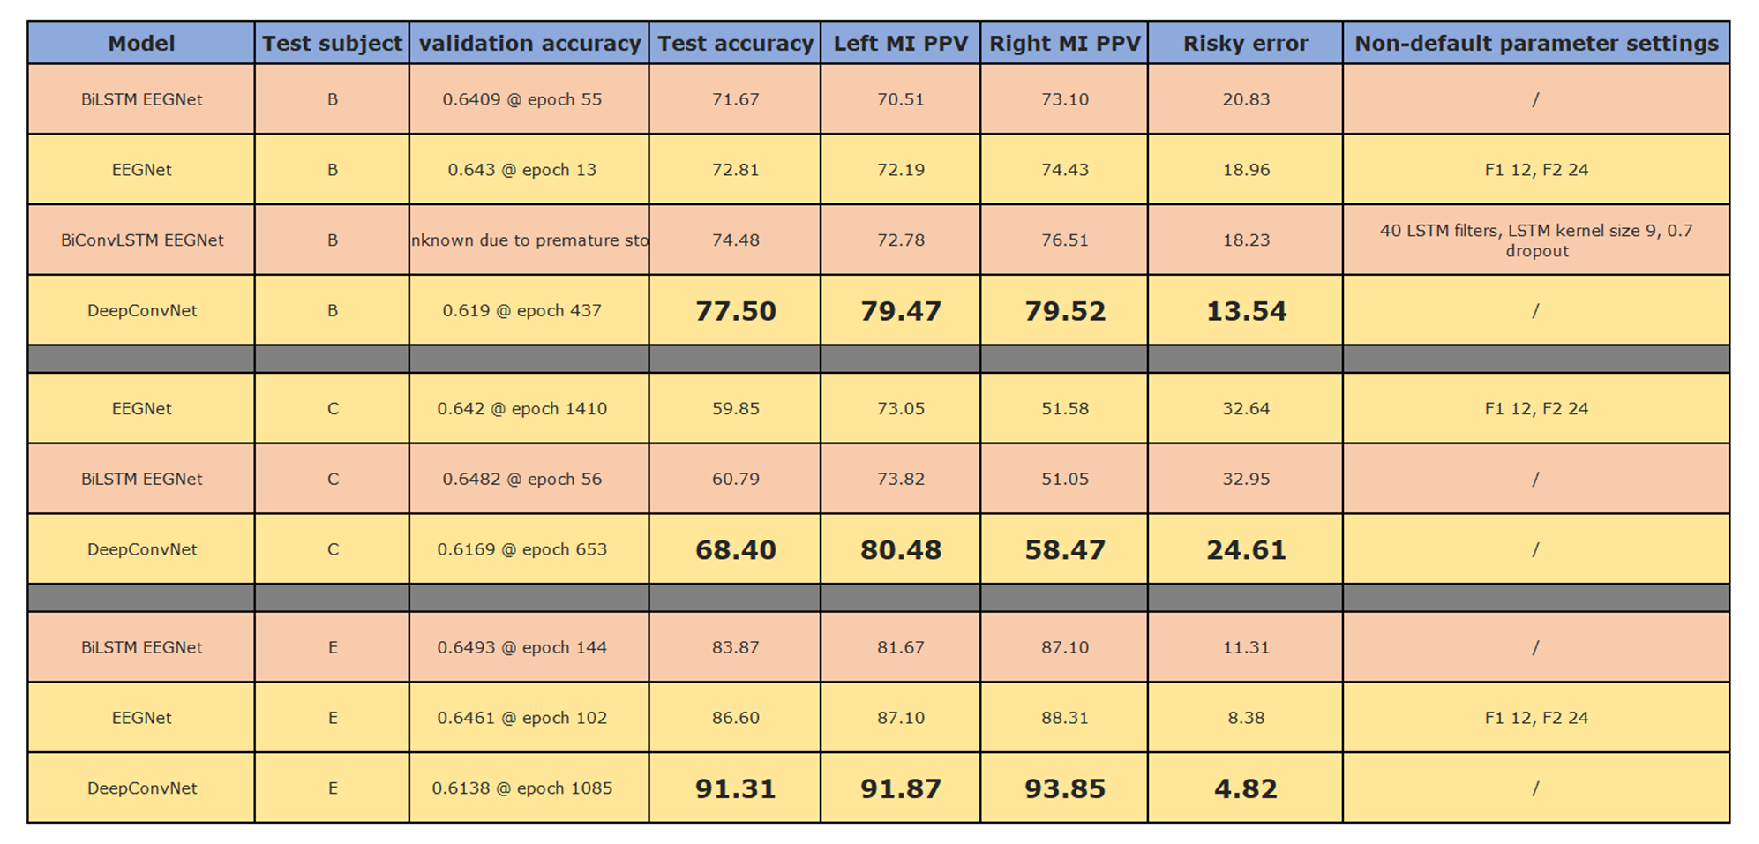
\includegraphics[width=\linewidth]{../images/results/more_data.pdf}
    \captionsetup{width=\linewidth}
    \captionsetup{justification=centering}
    \caption{Intersubject results for some of the one-step \gls{dl} classification approaches using more training data. Results are sorted based on the test subject and the obtained classification result on the test set. Colour codes denote either two-step \gls{csp} approaches, literature proposed \gls{cnn} approaches or master thesis proposed \gls{cnn}-\gls{lstm} approaches.} 
    \label{fig:results_more_data}
\end{figure}

The main experiments of this master thesis only made use of data from three of the provided subjects in the CLA dataset, as discussed in Section \ref{sec:evaluation_data_source}.
An additional pilot experiment was performed to test if adding more training data would increase intersubject performance.
Due to the increased data availability, this experiment setup did make use of a distinct subject for the validation split.
Figure \ref{fig:results_intersubject} summarizes all obtained results like before.
The added data gave significant improvement for all models without having performed additional hyperparameter tuning beyond logical reasoning.
The deepest \gls{cnn}, DeepConvNet, which now has access to sufficient data for training far outperforms all other \gls{dl} classification pipelines for all subjects.
This is not unreasonable given the other models were developed with a small dataset in mind \citep{eeg_model_eegnet}.
The results obtained from this intersubject experiment improve upon even the Intersession experiment results discussed in Section \ref{sec:evaluation_intersession}.

With a mean accuracy of $79.09$ ± $9.42$ DeepConvNet has a $77.50$\% accuracy for subject B and $91.31$ accuracy for subject E.
The latter could directly be used in an online bci setting where \gls{mi} tasks are expected on a known time interval.
The sharp contrast between subject C's test accuracy of EEGnet ($68.40$\%) and that of subject B also further illustrates how different brain signals can be between subject and session.
This pilot experiment provided very favourable results and it is clear that given enough data, deep networks such as DeepConvNet can generalise well.
The worse but still comparable results of EEGNet and its extensions proposed by this master thesis can be expected, as the shallow structure of EEGNet was made with the idea of having access to few samples in mind.
Further research building upon this work or dataset should therefore consider using all data available, perhaps even samples from the other interaction methods provided by \citet{eeg_data}, as these overlap in part with the CLA dataset and thus can provide even more information to classification pipelines.

% - - - - - - - - - -
% prediction time
% - - - - - - - - - -
\subsection{Comparison of prediction times}
\label{subsec:evaluation_pilot_studies_prediction_time}


When moving towards an online system where multiple overlapping sliding windows are likely to be used per second, the time it takes to make a prediction mustn't be too long as to cause issues for the often low-powered chip available in the processing hardware.
Since the one-step \gls{dl} models were most promising when looking at the experiment results, a small experiment was performed to test the prediction time of each proposed one-step \gls{dl} pipeline.
This was done by letting a trained model make the same 100 predictions 10 times.
Dividing this result by 100 gives the time needed per prediction and is less influenced by computational overhead caused by the timing functionality.
This experiment was then repeated a further ten times to obtain an idea of the variance of these estimates.
The results of this experiment are summarized in Figure \ref{fig:results_predict_time}, where the time in seconds needed to predict 1 sample of a 0.5-second long window is shown.

From this experiment, it becomes clear that besides slow training the bidirectional convolutional \gls{lstm} EEGNet extension is also more than 20 times slower in prediction time.
With a prediction time of over 0.1 seconds on a relatively capable system, it is unlikely that this model can be used for predicting sliding windows on a low-powered chip.
As such, a reconsideration of this model's complexity might be required when moving to an online system.
The other \gls{lstm} extended EEGNet model that was proposed in this master thesis did not suffer from this problem.

\begin{figure}[ht]
    \centering
    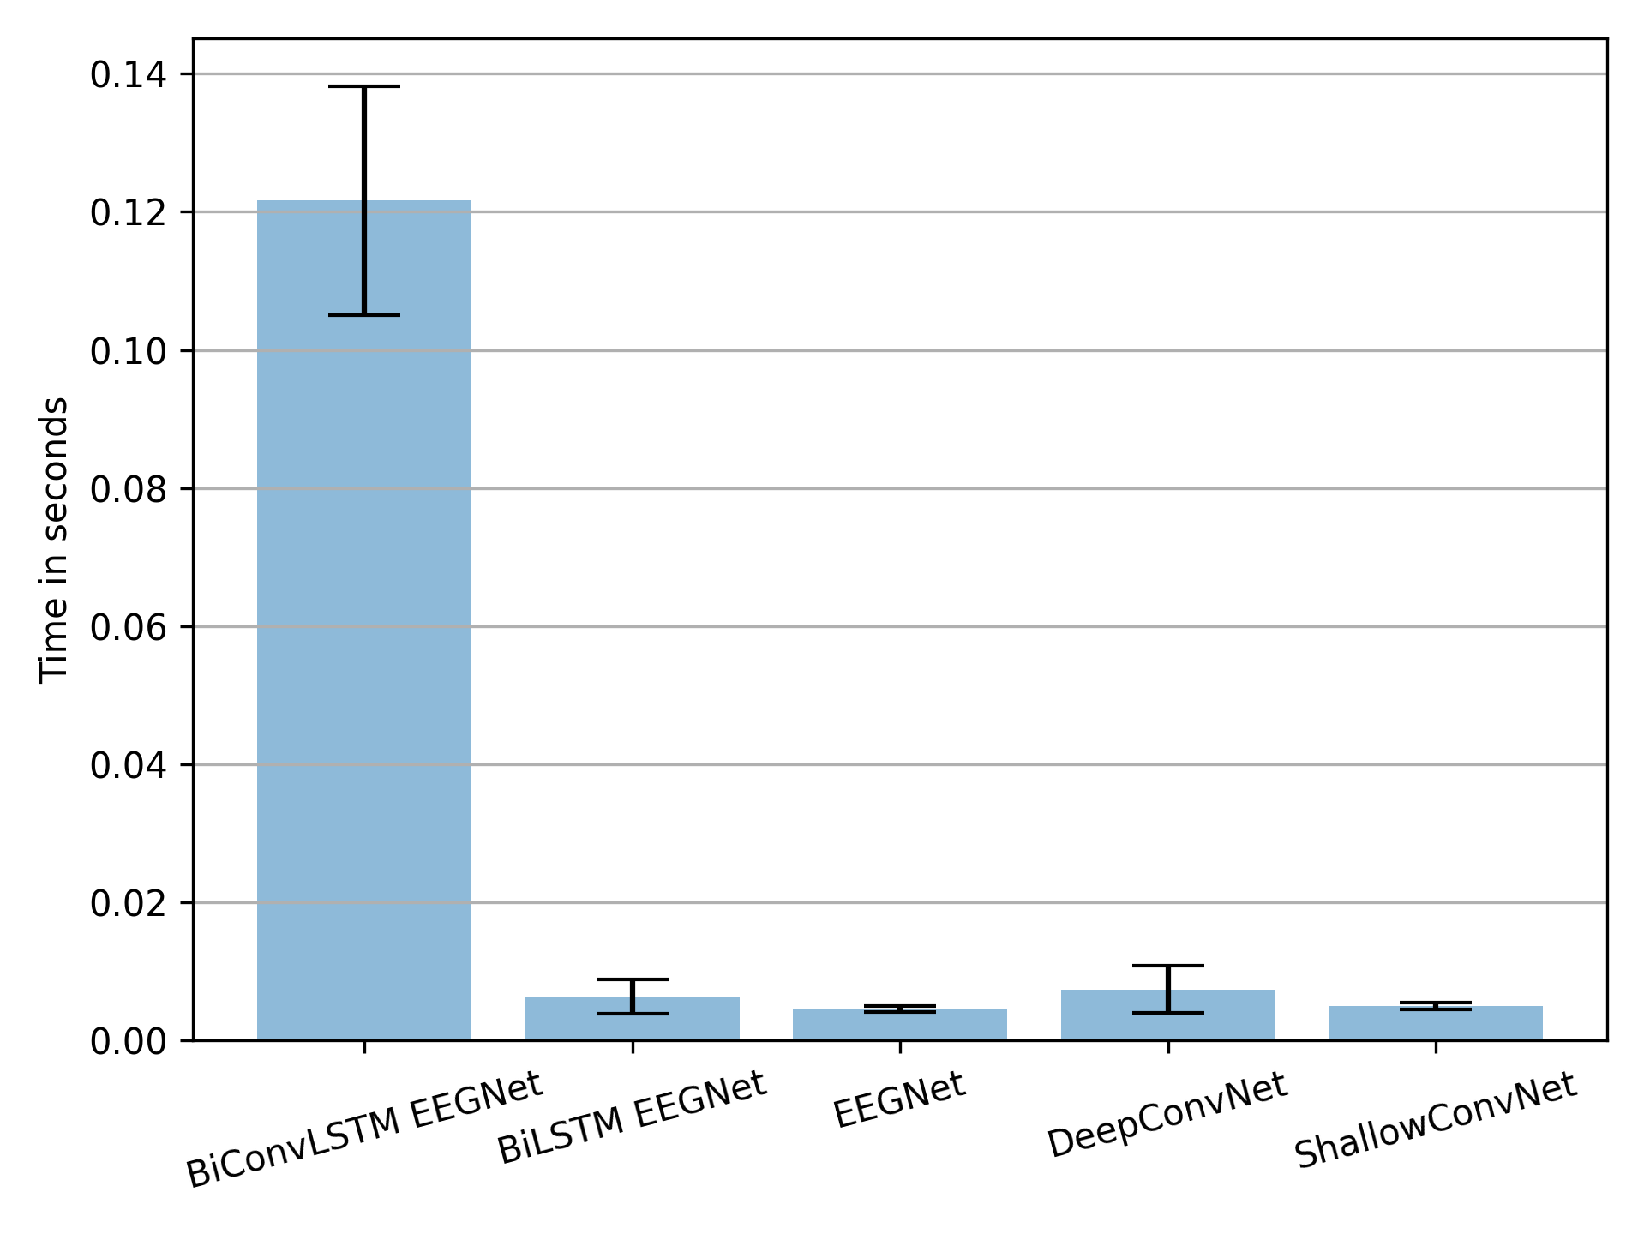
\includegraphics[width=0.6\linewidth]{../images/results/prediction_time.pdf}
    \captionsetup{width=0.6\linewidth}
    \captionsetup{justification=centering}
    \caption{Average prediction time in seconds for one 0.5 seconds long window with its standard deviation.} 
    \label{fig:results_predict_time}
\end{figure}


% - - - - - - - - - -
% other pilot
% - - - - - - - - - -
\subsection{Pilot studies with less promising results}
\label{subsec:evaluation_pilot_studies_others}

Besides the pilot studies already mentioned, the paper notebook 8 available on the GitHub of the master thesis also provides an initial pilot study on using \gls{csp} + LDA on \gls{mi} \gls{eeg} data where the electrodes were subsampled based on the proposals of Section \ref{subsec:biomedical_signals_working_with_eeg_anatomy}.
Whilst it has shown to be capable of producing similar results for subject B as those reported in this chapter, the generalisability to intersession or intersubject use of these traditional two-step \gls{ml} pipelines is not improved.
However, further studies to see if the one-step \gls{dl} methods can achieve comparable results using this subsampled channel selection should be made.
If so, this limits the dimensionality of the data considerably and will facilitate the learning process from a technical perspective and lower the prediction times reported in Section \ref{subsec:evaluation_pilot_studies_prediction_time}.

Another pilot study involved calibrating the \gls{dl} models on a new session by freezing the feature extraction layers and letting the fully connected layers learn further at a low learning rate using 5 minutes' worth of data.
Other variants of this freezing scheme were also used.
This produces mixed results as even with high dropout rates and regulations, the models seem to directly overfit on the new data samples and they do not boost the accuracy of the validation or test set by any significant means.
As discussed by \citet{eeg_model_eegnet}, most calibration done for \gls{mi} modelling has data available in the order of 20 minutes rather than 5.
Thus, using augmentation methods on the \gls{eeg} from 5 minutes might be a good approach to calibration using only a small amount of data.
\Citet{gan_eeg_augmentation} proposed the use of a \gls{gan} for this with promosing results.


% ---------------------------------------------- 
% Conclusions
% ---------------------------------------------- 
\section{Chapter conclusions}
\label{sec:evaluation_conclusions}

This chapter discussed the different experiments performed on the seven classification pipelines.
Three main evaluation paradigms were considered: intrasession, intersession and intersubject classification.
Besides accuracy, two other \gls{cm} derived metrics were used for reporting the classification results.
Thes additional metrics give insight into the models' performance for predicting labels that could be associated with risky actions in an online \gls{bci}.

When using a half-second window no statistically significant results were found that suggest the added memory provided by the \gls{lstm} layer benefits the classifier.
After discussing how this might be due to the data not being as prone to time shifts due to the use of a fixed windowing technique and a small window, a larger window was evaluated for the same three evaluation paradigms.
From this, it was found that the \gls{lstm} extended EEGNet model with a mean test accuracy of $65.52$ ± $0.89$, performed better than the regular EEGNet model which had a mean test accuracy of $60.68$ ± $1.64$ over all three subjects.
This suggests that the \gls{lstm} layer may still add increased capabilities to EEGNet, but that they require a different window strategy and further research to become better apparent.

Besides these main experiments, some pilot studies were also discussed.
One of these pilot studies showed that given enough data, deep \gls{dl} methods such as DeepConvNet can achieve more than 90\% classification accuracy for a three-class \gls{mi} problem in an intersubject evaluation paradigm.
These are great findings pushing towards further research to be done.
Some other potential promising extensions, such as reducing the complexity of the training by reducing the number of channels used and the use of augmented \gls{eeg} data for calibration, were also discussed but not favourably evaluated by the pilot experiments.
